\documentclass{article}
\usepackage[utf8]{inputenc}
\usepackage{algpseudocode}
\usepackage{amsmath}
\usepackage{algorithm}
\usepackage{tikz}
\usepackage{caption}

\title{The Course Registration Problem}
\author{Auden Woolfson}

\newcommand{\caps}{\operatorname{CAP}}
\newcommand{\sched}{\operatorname{SCHED}}
\newcommand{\ranks}{\operatorname{RANKS}}
\newcommand{\score}{\operatorname{SCORE}}

\begin{document}

\maketitle
\section{Introduction}
\setlength\parindent{0pt}\par
The initial idea of the course registration problem came from the stable matching problem. The stable matching problem is often conceptualized as a group of men and a group of women with equal cardinality, where the ultimate goal is to create a one to one matching where each agent has a partner of the opposite sex. Many of the principles pertinent to the stable matching problem remain with respect to the hospital-residents problem, which attempts to pair hospitals with medical students for residency. The key difference is that hospitals can pair with multiple residents, the exact number based on a variable capacity. Many to many stable matching is the problem where both sides can pair to multiple agents on the other side, which remains quite similar to the other two problems.\\\par

The course registration problem is fundamentally an extension of the many to many stable matching problem, modeling college students trying to register for the courses they want for the semester. Each course has a ranking of students that can include ties. This is because each student is ranked based on a priority function that can produce the same result for multiple students. This introduces types of stability, super, strong, and weak. For the purpose of this problem weak stability is completely adequate, and this goal will not change the nature of the problem greatly.\\\par

Another variation between the many to many stable matching problem and the course registration problem is that students have limited course rankings. This is because there are many courses that a student could prefer not be enrolled in any course than to be enrolled in (for instance, an English major in an advanced chemistry course). In most cases students would only be willing to take a small subset of the courses offered.\\\par

% unconfirmed

This difference does not impact the problem at all based on a simple reduction. A number of placeholder of "null" courses can be added to the course listings, each with capacity equal to the total number of registering students. Each of these courses will have a constant priority function for students, so all students are a tie. On each students preference list of courses each of the null courses will be placed in a set and constant order after the courses the student actually desires. There will always be enough space for students in these courses, and since all students are tied and prefer the courses in the same order it cannot result in a strong or super instability for a student to be enrolled in one of them. After the null courses on the preference list, students will have each of the other courses offered in any order completing the preference list, so that no stable matching will include students enrolled in them who do not desire to be. The version of the problem analyzed below has students with complete course rankings.\\\par

The final major difference and perhaps the greatest is the introduction of scheduling conflicts. Students may desire to be in enrolled in a course that has a scheduling conflict with another course that they would like to take if they are unable to enroll in the better one. This turns the course registration problem into a graph problem, where the offered courses represent vertices and an edge is placed between each pair of courses with a scheduling conflict. Students may only enroll in.\\\par

\section{Problem Definition}
\setlength\parindent{0pt}\par
Let $C$ be a set of $m$ course sections, and $S$ be a set of $n$ students\\\par
For each section $c \in C$ let $\caps_c$ denote the capacity of the section, let $\sched_c$ denote the list of times and days on which $c$ will be held\\\par
Let each $s \in S$ have a ranking $\ranks_s$ in order from most preferred to least preferred course by $s$, where $|\ranks_s| = |C|$, and there are no duplicates in $\ranks_s$ \\\par
Let $L$ be the maximum amount of courses a student can register for\\\par
For each possible pairing of some $s \in S$ and some $c \in C$, $(s, c)$, let there be a ranking score denoted by $\score_{s, c}$. This number is meant to represent the priority level of the student to get into that course, as opposed to the preference of the student. \\\par
Let $C_s$ denote the course sections some $s \in S$ is matched to and $S_c$ denote the students some $c \in C$ is matched to in an $S, C$ matching\\\par
Let an $S,C$ matching be considered valid if for each $s \in S$, $|S_c| \le L$, for each $c \in C$, $|S_c| \le \caps_c$, and for each $s \in S$, there exists no pair in $C_s$ with overlapping times ($\sched_c$)\\\par 

% work on this, stability is weird

Let an $S, C$ matching be considered stable if there are no rogue pairs. A rogue pair refers to a student that would prefer to be in a course that they are not enrolled in over one they have been enrolled in, where the pair of that student and course has a higher ranking score than some student enrolled in that course section. A rogue pair also refers to any student that would prefer to be in a section that they have not been enrolled in and still has space for more students, or a section with capacity for more students where some student would prefer to be in that section over one they have been enrolled in. Finally a rogue pair is any student and course section\\\par
Let a rogue pair be some $s' \in S$ and some $c' \in \ranks_{s'}$ in an $S, C$ matching where $|C_{s'}| \le L$, or if there exists some $c \in C_{s'}$ that is lower ranked than $c'$ in $G_{s'}$ (or does not exist in $G_{s'}$) that can be removed from $C_{s'}$ to meet the previous condition. The rogue pair also requires that $|S_{c'}| < \caps_{c'}$ or there exists a student $s \in S_{c'}$ where $\score_{s, c'} < \score_{s', c'}$. However, pairs that meet these conditions are not considered rogue if there is a time conflict between some $c \in C_s'$ and $c'$ where $c$ is ranked more highly in $\ranks_s'$ than $c'$\\\par

The goal is, given $S$ and $C$, produces a valid and weakly stable matching $X$.
\\\\

\section{Gale-Shapley Style Approach}

\begin{algorithm}
\caption{Assign students to sections using a Gale-Shapley style approach}
\begin{algorithmic}[1]
\Procedure{Assign Students}{$S$, $C$}
\State $freeStudents \gets S$
\While{$freeStudents$ is not empty}
\State $s \gets freeStudents[-1]$
\While{$s$ has not proposed to some section in $\ranks_s$\par
\hskip\algorithmicindent that has no time conflict with any section in $C_s$\par 
\hskip\algorithmicindent and $|S_c| < L$}
\State $c \gets$ first section in $\ranks_s$ that $s$ has not proposed to\par
\hskip\algorithmicindent\hskip\algorithmicindent and does not conflict with any section in $C_s$
\State mark $c$ as proposed to in $\ranks_s$
\If{$|S_c| < \caps_c$}
\State Append $s$ to $S_c$
\ElsIf{$\score_{s,c} > (\score{s',c} | s' \in S_c$)}
\State $s' \gets$ the student in $S_c$\par
\hskip\algorithmicindent\hskip\algorithmicindent\hskip\algorithmicindent where $\score_{s',c}$ is the lowest of any possible $s' \in S_c$
\State remove $s'$ from $c$
\State Append $s$ to $S_c$
\If{$s'$ is not in $freeStudents$}
\State Append $s'$ to $freeStudents$
\State \textbf{break}
\EndIf
\EndIf
\EndWhile
\If{all entries in $\ranks_s$ have been marked as proposed to\par
\hskip\algorithmicindent or conflict with sections in $C_s$\par
%this can be done because the student will be added back to free students if %they are kicked out and will get the opportunity to propose again
\hskip\algorithmicindent or $|S_c| \ge L$}
\State pop $s$ from $freeStudents$
\EndIf
\EndWhile
\State Add all current student section pairs to an $S, C$ matching $X$
\State\Return $X$
\EndProcedure
\end{algorithmic}
\end{algorithm}
\break

First, it can be proven that this algorithms will always return a stable matching in a case with no time conflicts between sections. Then it can be shown how this approach fails when time conflicts are introduced.\\

In a scenario with no time conflicts, students will "propose" to each course in their ranking in the order of the ranking with no exceptions. Assume towards contradiction that in this scenario, the algorithm produces a matching that includes a rogue pair and is therefore not pairwise-stable. Let an example of this pair be called ($s$, $c'$) where $S_c'$ includes a student $s'$, $\score_{s',c'} < \score_{s,c'}$ and $C_s$ includes some course section $c$ that is lower in $\ranks_s$ than $c'$.\\

Since $c$ is in $S_c$, $s$ had to have "proposed" to $c'$ before proposing to $c$, and since $c'$ is higher in $\ranks_s$ than $c$, $s$ must have either been rejected by $c'$ initially or removed in favor of another student with a higher score. In the case of an initial rejection, $S_c'$ must have already been full of students with higher scores than $s$. Since full course sections can only accept students with higher scores than some student that has already enrolled, it would be impossible for this condition to then change and impossible for $(s, c')$ to be a rogue pair. In the case of a removal of $s$ from $S_c'$ in favor of another student $s$ must have been the lowest scoring student in $S_c'$. After being replaced, $s$ would have a lower score than any student in $S_c'$. This is the same condition that occurs in the case of an initial rejection, and makes it impossible for $(s, c')$ to be a rogue pair.\\

Since a rogue pair is impossible if the student has already "proposed" to the course section, and the student must have already "proposed" to the course section, a rogue pair cannot be produced in a matching created by the algorithm on inputs without any time conflicts within students course selections.\\

Note that in this problems definition of rogue pair, an $(s, c')$ pair is not rogue if the student is matched with another course $c$ where $c$ is higher in $\ranks_s$ than $c'$ and $\sched_c$ and $\sched_{c'}$ have some overlap (time conflict).\\

Time conflicts introduce a new potential way for a rogue pair to arise in a matching. A student may not be enrolled in a course section due to time conflict, but may still prefer it to some other section they are enrolled in while scoring higher than some other student enrolled in said section.\\

One way for a rogue pair to arise in a scenario with time conflicts involves a student that has ranked conflicting courses, that do not all conflict. Consider some student $s$ where $\ranks_s$ includes course sections $a$, $b$, and $c$ in that order. $a$ and $b$ have conflicting schedules and $b$ and $c$ have conflicting schedules, but $a$ and $c$ do not. $s$ may initially be able to enroll in $a$, which will stop $s$ from proposing to $b$. Since there is no conflict between $a$ and $c$, $s$ can then enroll in $c$. If some student $s'$ then proposes to $a$ and $\score_{a,s'} > \score_{a,s}$, $s$ will be removed from $a$ if it is at capacity. In this scenario $s$ never gets the opportunity to propose to $b$ despite $b$ being first in $\ranks_s$. If $S_b$ is populated with students that score lower than $s$ for $b$, $(s, b)$ will be a rogue pair. \\

\begin{figure}
  \centering
  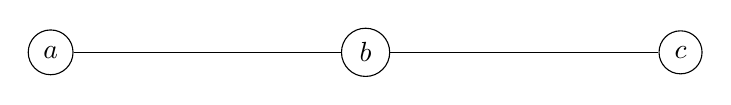
\begin{tikzpicture}[scale=2] % Adjust the scale factor to make the graph larger
    % Nodes
    \node[circle, draw] (a) at (0,0) {$a$};
    \node[circle, draw] (b) at (2,0) {$b$};
    \node[circle, draw] (c) at (4,0) {$c$};

    % Edges
    \draw (a) -- (b);
    \draw (b) -- (c);
  \end{tikzpicture}

  \begin{itemize}
  \item \(\ranks_{s}\): $a, b, c$
  \item \(\score_{a, s}\): 1
  \item \(\score_{a, s'}\): 2
  \end{itemize}
  
  \caption{The graph represents the case where scheduling conflicts can result in a rogue pair.}
  \label{fig:graph}
\end{figure}

The immediate thought for fixing the problems that may arise when this case exists while staying inside the Gale-Shapley framework is to have $s$ propose to $b$ immediately after being removed from $a$, and simply leave $c$ if they are able to enroll. This would in fact eliminate the possibility of $s$ from being in a rogue pair, however this approach creates a new issue. If $s$ is to leave $c$, some student $s''$ may have already proposed to $c$ and failed to enroll because the capacity was full and all students have a higher score. If no other student with a higher score than $s''$ fills the new vacancy in $c$ where $s$ was, $s''$ and $c$ will be a rogue pair. This case makes it impossible to guarantee a stable matching from this algorithm.

\end{document}